

The aim of this chapter is to provide the required clinical background on breast cancer screening and diagnosis for a good understanding of the global aim and relevance of the present work. 

First the breast evolution from early to the adult ages is described, with a detailed characterization of internal and external adult breast structures. To explain the intra-individual variation of breast mechanical and structural properties, the hormonal changes during the menstrual cycle, pregnancy or menopause are presented.   Next the cancer edogenesis is described and the most common types are characterized. Finally, different modalities for breast imaging are presented with their underlying technical principles as well as their relevance for breast cancer regular screening.

\clearpage
\section{Breast anatomy}\label{section:breastanatomy}

Internal and external breast structures will be repeatedly referenced in the following work, therefore their detailed description including mechanical properties and their localization is needed. Although the breast anatomy seems to be simple and easy to understand, a detailed analysis of breast embryogenesis is requested for a better localization of the supporting breast tissues. The breast support matrix is a structure of high interests when modeling breast mechanics.  

  
\subsection{Breast embryogenesis}\label{subsection:breastembryogenesis}

The breast is a modified skin gland which starts to develop at the embryonic stage from the epidermis and dermis.  During the sixth fetal month, from 12 to 20 solid cords of epithelial cells are growing down into the dermis (Figure. \ref{breastembryogenesis}.a-b). Later, these cords evolve into lactiferous ducts and alveoli (fig. \ref{breastembryogenesis}.c-d). Thus, near birth, a simple network of branching ducts is already developed in the pectoral area \citep{skandalakis_embryology_2009}.
 

 \begin{figure}[!h]
 \centering
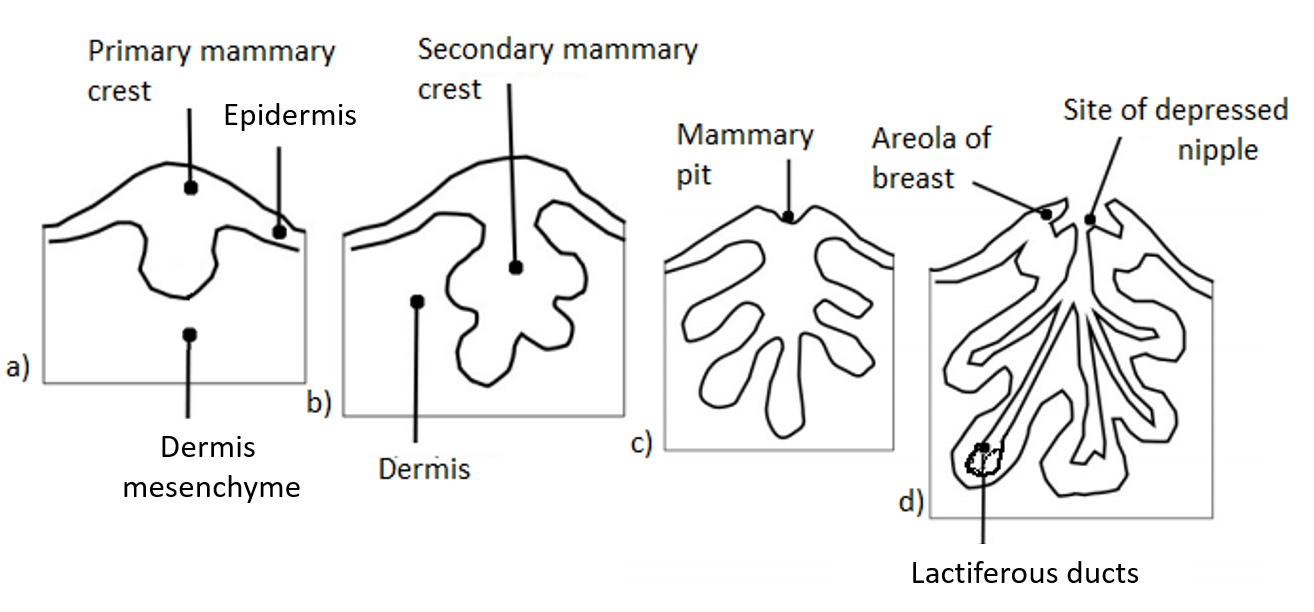
\includegraphics[width=0.8\textwidth,keepaspectratio]{figures/breast_evolution_my.png} 
\caption[Breast embryogenesis] {Breast embryogenesis: stages of formation of the duct system. the ectoderm is responsible for duct system and alveoli, the mesenchyme is responsible for the connective tissue and vessels \citep{skandalakis_embryology_2009}.}
\label{breastembryogenesis}
\end{figure}


The glandular lobes, generally remain underdeveloped until puberty (13 to 18 years). Under hormonal stimulation, the breast buds due to the development of the mammary glands and increased deposition of fatty tissues, become palpable discs beneath the nipple. The ducts grow into the soft tissues and the lobular differentiation begins \citep{kopans2007breast}. 

\cite{kopans2007breast} analyzed breast development sequence in the subcutaneous tissues. According to the authors the evolution of breast within the fascial system is unclear, with two possible evolution paths: 
\begin{enumerate}[label=(\Alph*)]
\item The superficial fascia splits in two layers forming the deep and the superficial fascia layers. The mammary glands appears between these two layers (Figure\ref{breastevol_fascia}.A).
\item The elongating ducts retracts the superficial fascia.  The mammary glands is enveloped by the superficial fascia (Figure\ref{breastevol_fascia}.B)
\end{enumerate}

\begin{figure}[!h]
\centering
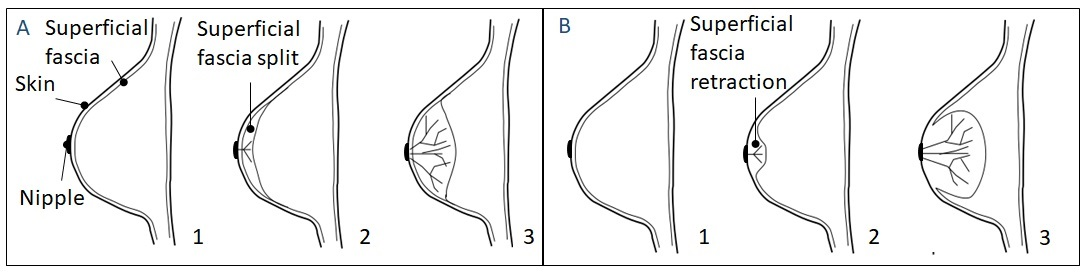
\includegraphics[width=0.9\linewidth,keepaspectratio]{figures/breastEvol_fascia_my.jpg} 
\caption[Breast development sequence into subcutaneous tissues.]{Breast development sequence in the subcutaneous tissues. A) Mammary bud development by splitting the superficial fascia in 2 layers. B) Mammary bud development by fascia retracting, reproduced from  \citep{kopans2007breast}. }
\label{breastevol_fascia}
\end{figure}


\subsection{Breast external appearance}\label{subsection:breastappearance}

In order to describe the breast appearance, several notions for localization into the breast volume and its vicinity are defined. Usually, the breast volume is divided into four quadrants: upper outer quadrant (UOQ)\nomenclature{UOQ}{Upper Outer Quadrant}, upper inner quadrant (UIQ)\nomenclature{UIQ}{Upper Inner Quadrant}, lower outer quadrant (LOQ)\nomenclature{LOQ}{Lower Outer Quadrant}, lower inner quadrant (LIQ)\nomenclature{LIQ}{Lower Inner Quadrant}(see Figure \ref{fig:Breast_quadrants_full}). On the other hand, the anatomical structures surrounding the breast are localized using the anatomical landmarks such as  the inframammary fold, the clavicle, the sternal angle, the sternal line, the costal margin and the axilla.

\begin{figure}[h]
\centering
 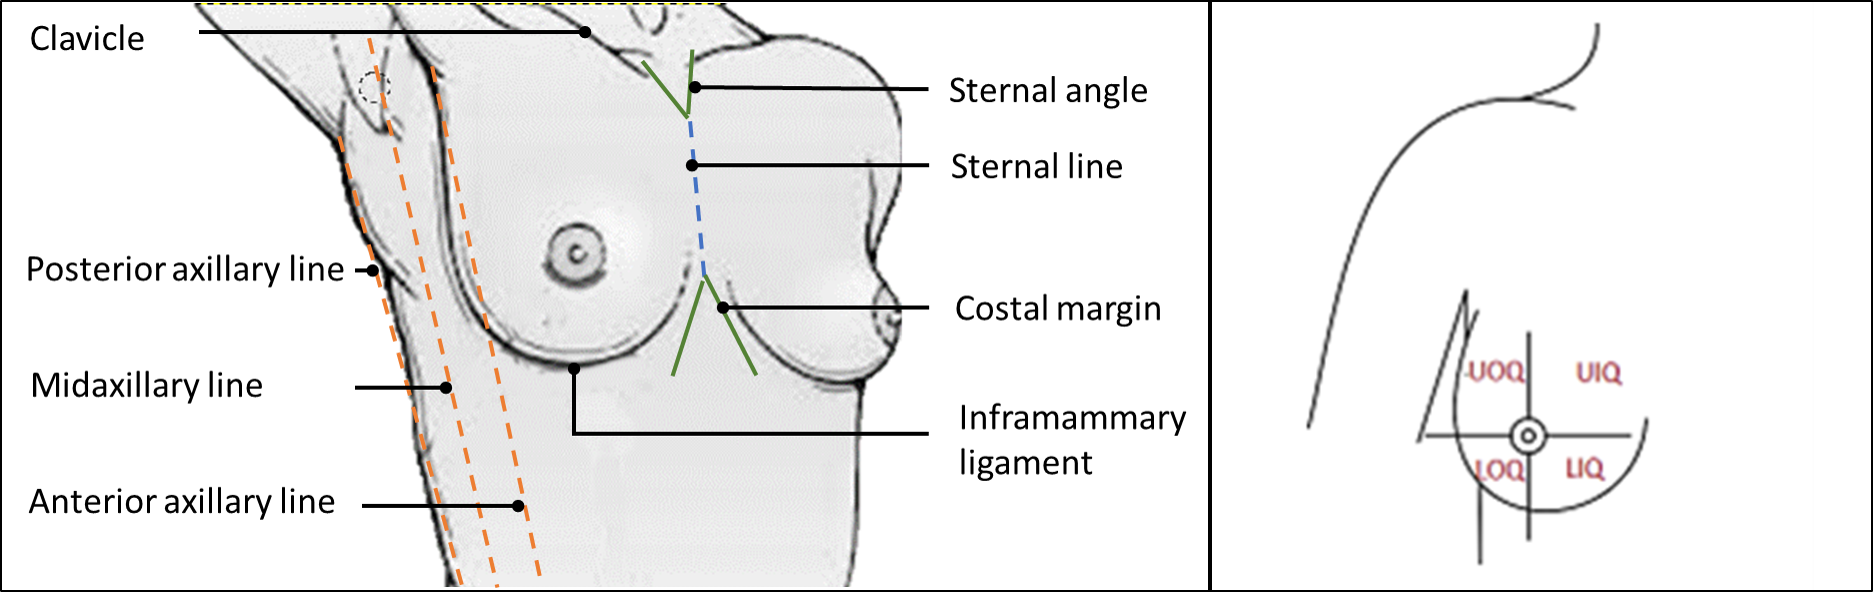
\includegraphics[width=\textwidth,keepaspectratio]{figures/Breast_quadrants_full.png}
  \caption{Left: thorax landmarks; Right: four breast quadrans \citep{vandeput2002considerations}}\label{fig:Breast_quadrants_full}
\end{figure}


 Anatomically, the adult breast is localized on top of the ribcage, between the clavicle superiorly and costal margin inferiorly. Its transverse boundaries are defined from the sternal line medially to the midaxillary line laterally (Figure\ref{fig:Breast_quadrants_full}). The intra-individual asymmetry (between left and right breasts) is considered as a normality for the young and the adult breast . The breast shape and contour are influenced by \citep{mugea2014aesthetic}:
 \begin{itemize}
 \item The volume of mammary gland in each breast quadrants.
 \item The amount of the subcutaneous and intra-lobular fat.
 \item The body contour of the chest wall.
 \item The muscular covering and thickness.
 \item The thickness and elasticity of the skin.
 \end{itemize}

Anthropomorphic characteristics of women breast were studied almost for the aim of cosmetic and reconstructive surgery.  \cite{vandeput2002considerations} measured distances between anatomical landmarks of the thorax of 973 women with aesthetically near-perfect breasts. The authors proposed different relations as guidelines to compute the recommended breast size parameters (nipple-mid clavicle distance, nipple inframammary fold distance) as a relation of body parameters (body height, torso width). In their study, a poor correlation was found between body height or weight and breast volume. Contrariwise a high correlation was found between the nipple to  inframammary fold distance or the nipple to mid clavicle distance and the thorax width. \cite{catanuto2008experimental} mentioned that the breast shape after surgery cannot be predicted by volumetric measurements only; they have proposed additional measures (areas, distances or angles) allowing unambiguous characterization of the breast shape. According to the authors, the curvature of the thoracic surface is the most relevant parameter to evaluate the outcome of a reconstructive breast surgery.
 
Starting with the Warner Brother Corset Company in 1935, the underwear industry introduced a new unit to measure the breast volume, the cup. The cup size is computed using a relation between the circumference of the chest at the level of the nipples and the torso width \citep{pechter_new_1998}.

\subsection{Internal structures}\label{subsection:internalstructures}

Breast heterogeneous structure includes a mixture of parenchyma and adipose tissue (Figure \ref{fig:breastanatomy}). The breast parenchyma consists of glandular components, lymphatic network and blood vessels \citep{clemente2011anatomy}. Skin, Cooper's ligaments and fascias are the supporting system of the breast; their interconnection and intersections with the pectoral muscle fix and support the breast soft tissues \citep{mugea2014aesthetic}.

The \textbf{ adipose tissue} is the predominant tissue of the breast that fills up depressions between the deep and superficial fascia. In the intra-fascial space, adipose tissue surrounds and is dispersed among the glandular structures. Fat properties and its spatial distribution give the breast a soft consistency. The main aim of this tissue is to protect the lobes and lactiferous ducts.

The \textbf{ glandular tissue} is represented by breast lobes. A healthy female breast is made up of 12-20 lobes. They are distributed centrally and laterally within the breast. The total amount of glandular tissue depends on the hormonal fluctuation, age and physical state.  Mammary ducts arise from the lobes as branches and connect them to the female nipple. There are about 10 duct systems with a tree-like structure in each breast that carry the milk from the lobes to the nipple. The dark area of skin surrounding the nipple is called the areola.

 \cite{huang2011characterization} have studied the breast shape and fibro-glandular distribution using dedicated breast CT images. This study shows that the glandular tissues is situated in the central portion of the breast. In prone position about 60 $\%$ of glandular tissues is located near to the nipple. A mean percentage of glandular tissue was computed by \cite{yaffe2009myth}, the values varied from 13.7$\%$ to 25.6 $\%$ within different groups. They also mentioned a drop in glandular fraction with the advancing age. 


\begin{center}
\begin{figure}[h]
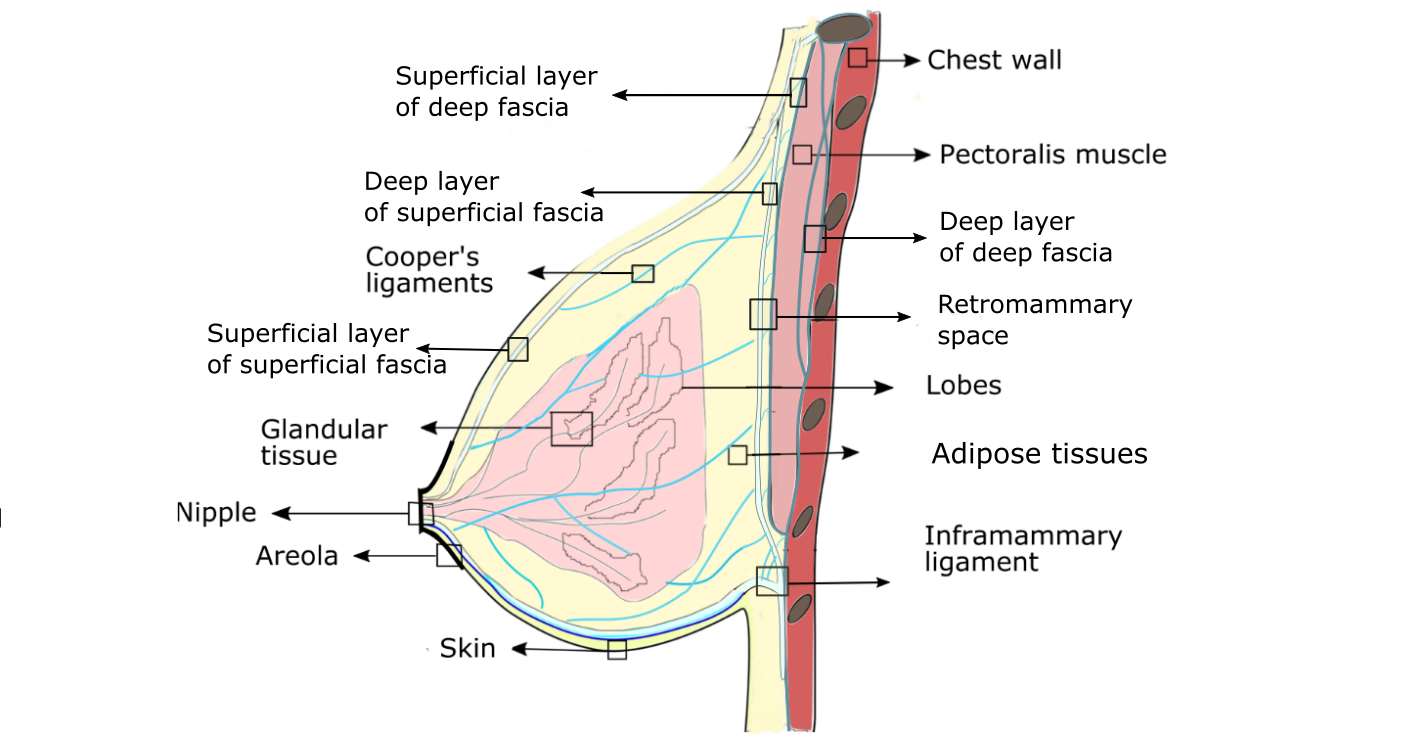
\includegraphics[width=\textwidth,keepaspectratio]{figures/anatomieSeinEuBlack2.png} 
\caption{Breast anatomy, \citep{clemente2011anatomy}}
\label{fig:breastanatomy}
\end{figure}
\end{center}

 A layer of adipose tissue and connective fascia separates the breast from the pectoral muscle forming a retro-mammary fat space.
 
The \textbf{skin} is the covering breast layer which provides protection and receives sensory stimuli from the external environment. It is a heterogeneous organ composed of 3 layers (see Figure \ref{fig:skinanatomy} , \citep{kanitakis2002anatomy} ): epidermis (dead cells) mainly composed of keratin, dermis composed of collagen and elastin fibers in a viscous matrix made of water and glycoproteins and hypodermis, mainly composed of adipocytes cells.


\begin{figure}[!h]
\centering
\centerline{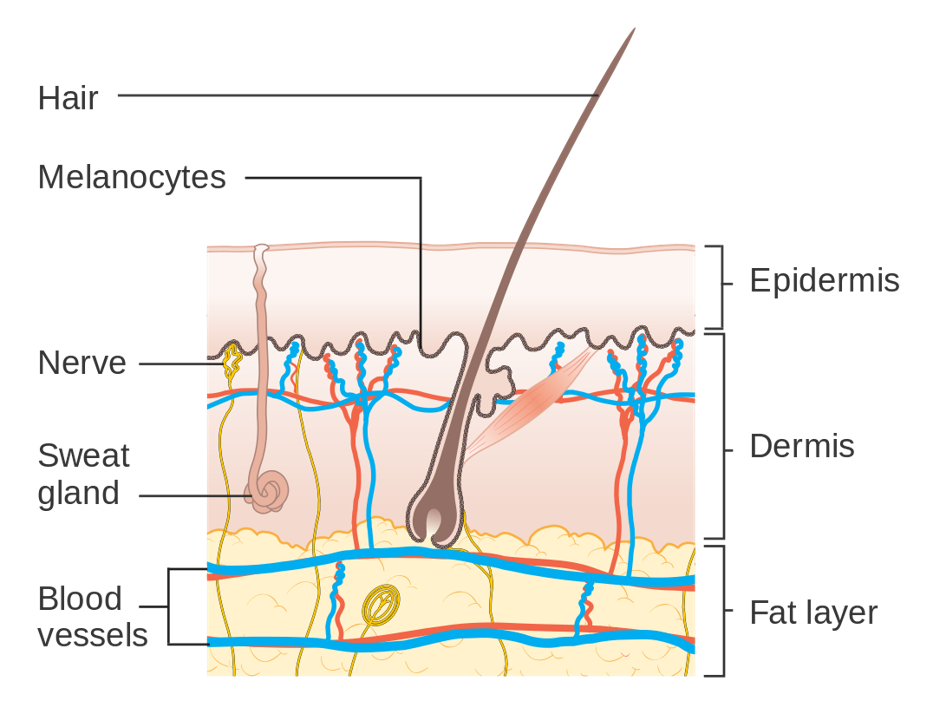
\includegraphics[width=0.5\textwidth,keepaspectratio]{figures/skin_2.jpg} }
\caption{Skin anatomy, \textit{Cancer Research UK}}
\label{fig:skinanatomy}
\end{figure}



The breast skin thickness vary from beast base to the nipple between $\sim$ 2 $mm$ and $\sim$ 0.5 $mm$. At the nipple areola region, the skin thickness measure 4-5 $mm$.
 \citep{andolina2011mammographic}. \cite{sutradhar_vivo_2013} studied the breast skin thickness of 16 different sectors radially oriented around the nipple. The thickness range proposed by the authors varies between $0.83 mm$ and $2.35 mm$ with a mean of $1.55 \pm 0.25 mm$. According to this study, the skin thickness varies as follows: the lateral
region thickness is the thinnest among all the breast regions followed by superior/inferior and medial region; there is no significant difference between the inferior and superior breast regions; in the radially exterior region, the skin is thicker than in the radially interior region (close to the nipple).  \cite{ulger2003effect} found that, during the breast puberty, the breast volume increases and the skin thickness decreases in all regions.

The \textbf{connective tissue} is represented by Cooper's ligaments and fascial system. The breast fascial system is composed of deep fascia and superficial fascia. During puberty, breast is growing and the superficial fascia divides in two layers: the deep layer of the superficial fascia and the superficial layer of the superficial fascia \citep{kopans2007breast}.  Cooper's ligaments run throughout the breast tissue parenchyma from the deep layer of the superficial fascia beneath the breast to the superficial layer of superficial fascia where they are fixed (Figure \ref{fig:breastanatomy}). Because they are not taut, these ligaments allow the natural motion of the breast \citep{clemente2011anatomy}. Between the deep layer of the superficial fascia and the superficial layer of the deep fascia, a layer of connective loose tissue forms the retro-mammary space, allowing the breast tissue to slide over the chest \citep{mugea2014aesthetic}. In regions where the superficial fascia meets the deep fascia, suspension ligaments are created. One of these ligaments is situated at the level of the sixth and seventh ribs and is called the \textbf{inframammary ligament} \citep{bayati_inframammary_1995}. It evolves into the \textbf{deep lateral ligament} and the \textbf{deep cranial ligament} that are respectively attached to the axillary fascia and to the clavicle. The second meeting point of the 2 fascias is situated on the sternal line and is called the \textbf{deep medial ligament} (Figure \ref{fig:suspensoryligaments}). On the upper pole of the breast, near the second rib space, the deep fascia tightly connects with the 2 layers of the superficial fascia, here the third meeting point is created. The three ligaments are 3D structures, evolving from pectoral muscle toward the nipple underlying the skin surface.


The existence, the topography, and the thickness of the membranous layers of the superficial fascia have been studied in various regions of the body \citep{abu_membranous_2006}. According to the authors, the thickness of these superficial layers in both superior and inferior breast regions is equal to $88.12 \pm 7.70 \mu m$ and $140.27 \pm 11.03 \mu m$ respectively.

\begin{figure}[!h]
\centering
\centerline{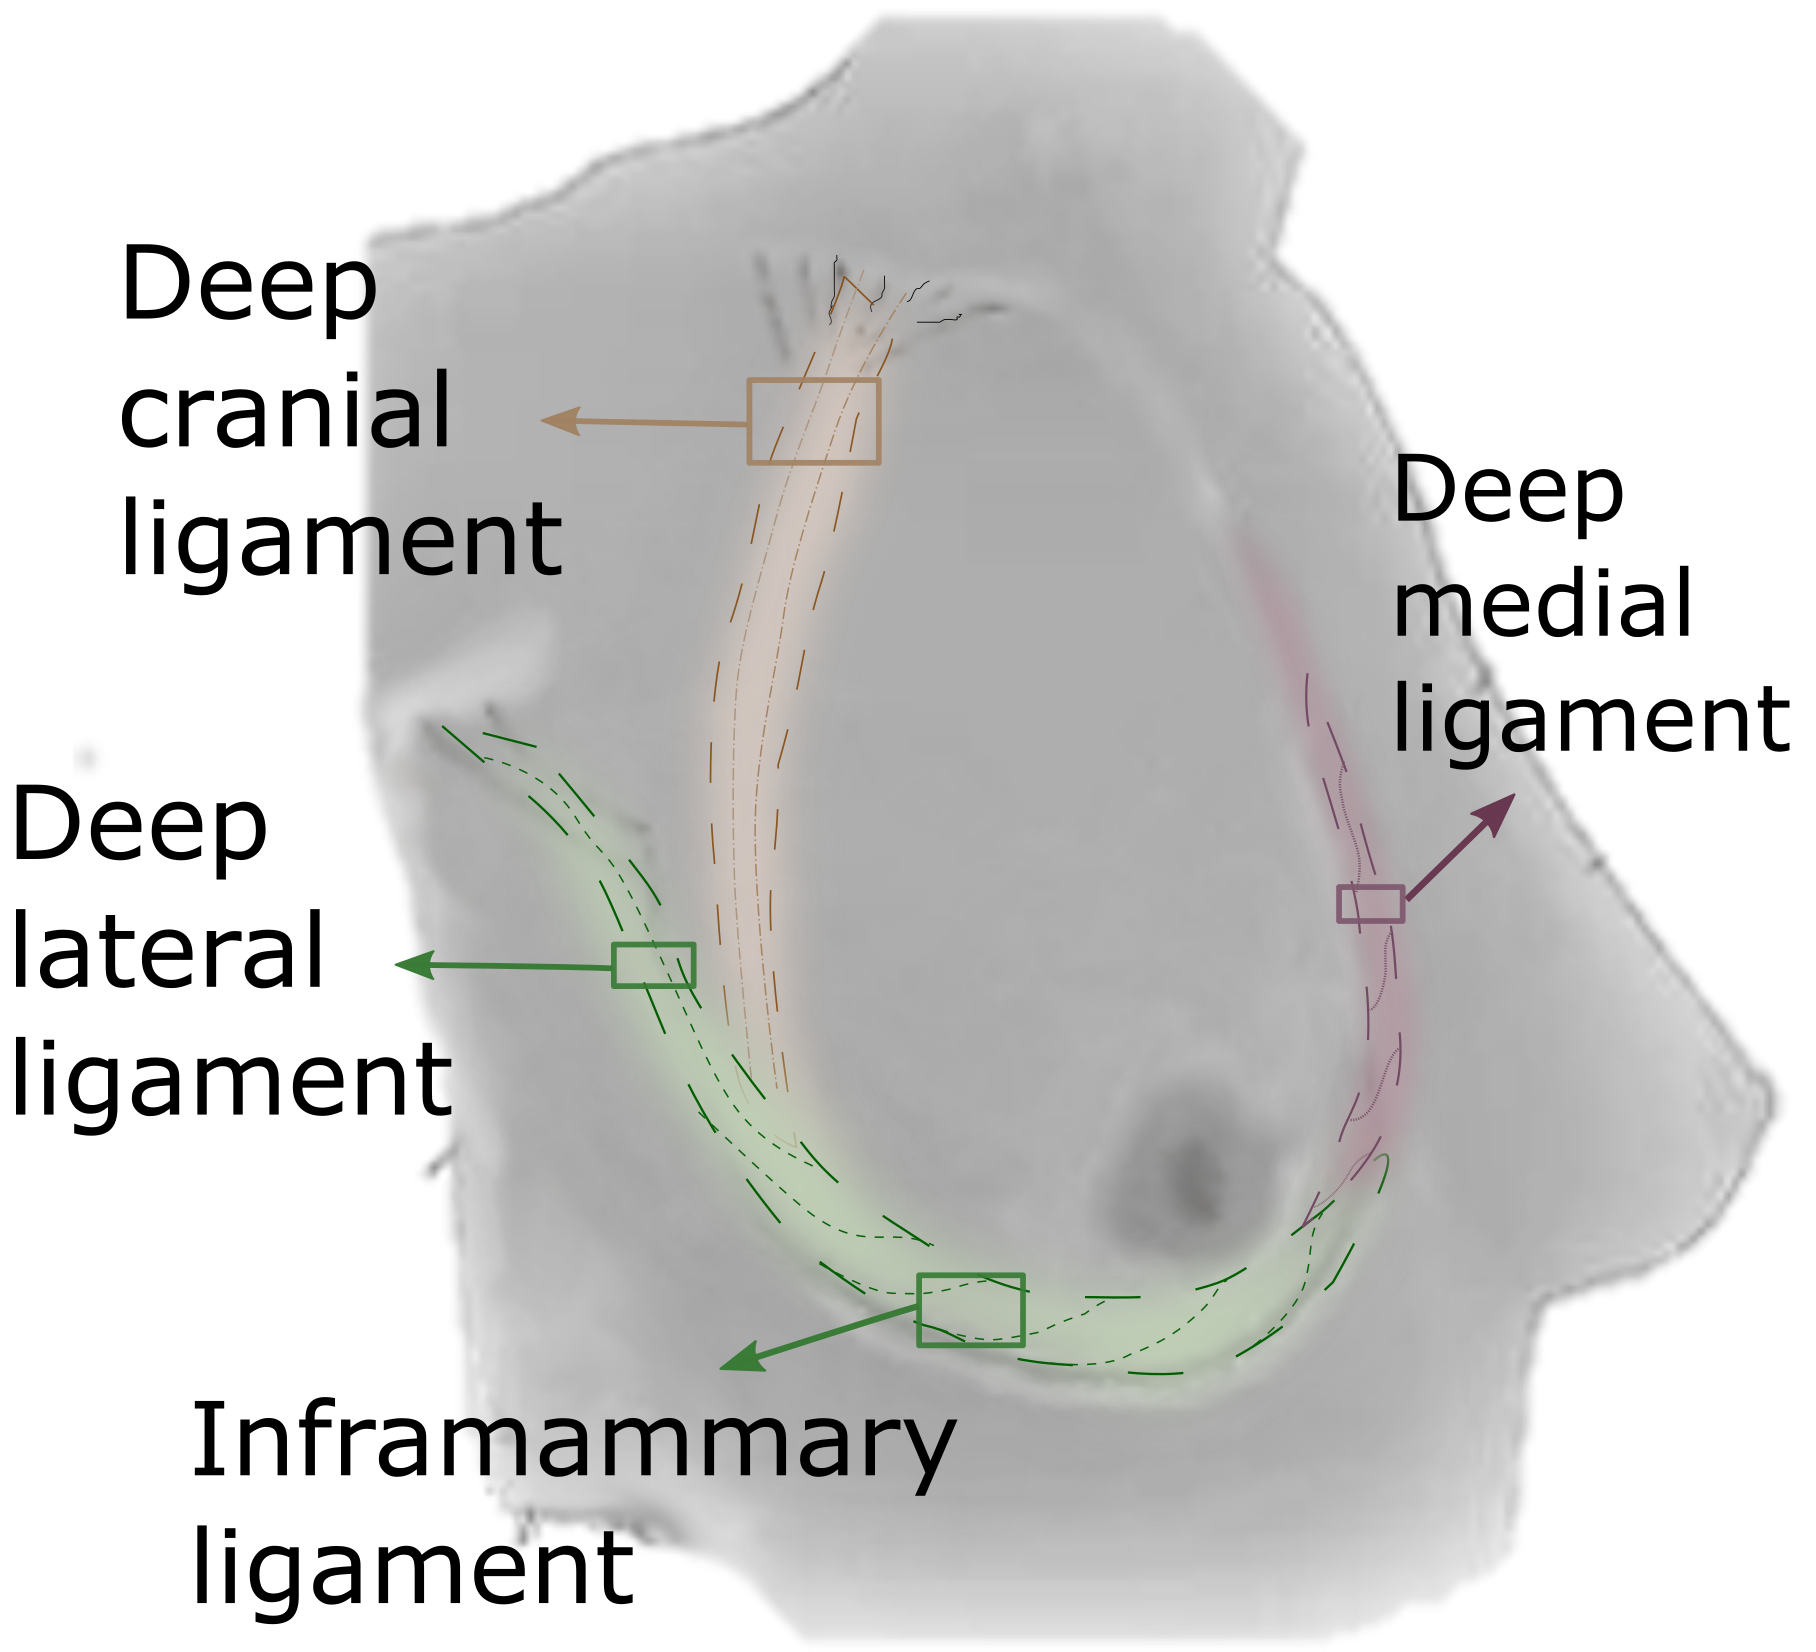
\includegraphics[width=0.4\textwidth,keepaspectratio]{figures/breastLigaments.png} }
\caption{Suspensory ligaments. The suspensory ligaments together with the fascias constitute the breast sport matrix and ensure the tissues inter-connection.   \citep{mugea2014aesthetic}}
\label{fig:suspensoryligaments}
\end{figure}


The lymphatic system is a vessel network which insures the transportation of white blood cells from tissues into the bloodstream.  All intramammary lymph nodes are located in the lateral half of the breast along the margin of the breast parenchyma  \citep{kopans2007breast}.  The lymphatic drainage of the breast extends from the subareolar plexus deep to and around the nipple (Figure \ref{fig:lyphaticDrainageandArtery} ).

The blood supply to the breast comes primarily from the internal mammary artery named successively subclavian, axillary, and brachial arteries (Figure \ref{fig:lyphaticDrainageandArtery}). From them, the lateral and internal thoracic arteries runs underneath the main breast tissue.

	
\begin{figure}[!h]
\centering
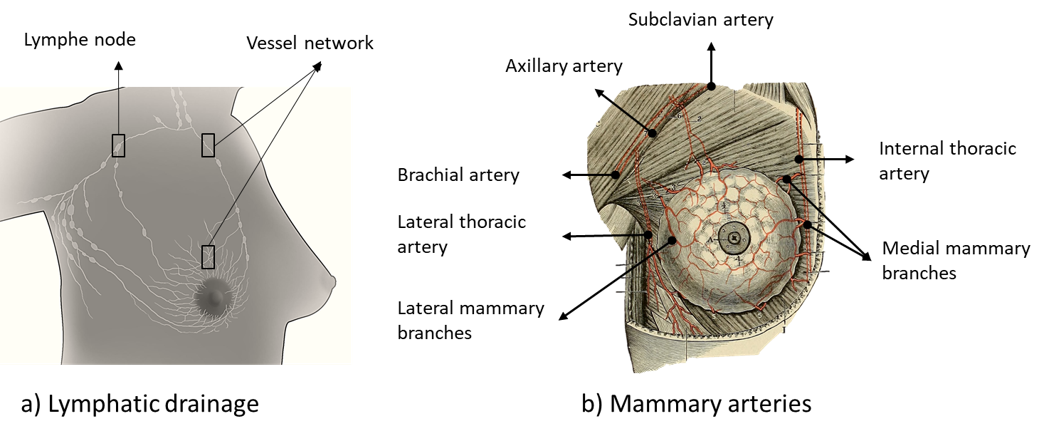
\includegraphics[width=\textwidth,keepaspectratio]{figures/lyphaticDrainageandArtery.PNG} 
\caption[Lymphatic system and Mammary Arteries for adult female breast. ]{Lymphatic system and Mammary Arteries for adult female breast.  Images reproduced from \cite{NCI_2012} and \cite{pilcher_breast_1917}}
\label{fig:lyphaticDrainageandArtery}
\end{figure}





\subsection{Adult breast texture changes}\label{subsection:adultbreasttexturechanges}

The female breast undergoes substantial changes during the woman's lifetime.  Most changes are caused by hormones and by woman's physiological condition. Important changes in female breast stiffness and composition occur during the menstrual cycle, pregnancy and menopause. 

There are 3 important phases during the menstrual cycle caused by hormonal fluctuation \citep{andolina2011mammographic}. During the first phase, the estrogen (hormones) diffusion stimulates the epithelial cell multiplication and the enlargement of ductal structures. Next, during ovulation, epithelial cells begin to grow in the lobule due to progesterone hormone; an increase in blood flow is also noticed. In the last phase, the ductal structures and the lobes support an involution and a regression process. It must be mentioned that not all lobules regress, therefore during menstrual cycle new lobules can be created.   The work by \cite{lorenzen_menstrual-cycle_2003} showed that, during the premenstrual phase the stiffness of fibro-glandular tissue and glandular tissue can change by 30\% and 14 \% respectively. They also have shown that in the middle of the menstrual cycle, the parenchyma volume increases of 38\% and the water content by 24.5\%.

During pregnancy, under the influence of estrogen and progesterone, the breast enlarges in volume and density, the veins dilate and the proportion of parenchyma tissues increases.  When lactation is weaned the breast returns to the pre-pregnancy state, and the atrophy of glandular, ductal, and stromal elements  is observed \citep{pandya_breast_2011}.

The menopausal breast contains a larger fraction of fatty tissues and reduces the number of ductal and lobular elements. During the first four years after menopause, the breast is the subject of an atrophy process. The atrophy begins medially and posteriorly, then laterally, working its way to the nipple \citep{andolina2011mammographic}. In this period the breast loses progressively fat and stoma tissue, resulting in breast shrinkage and loss of contours.

 The breast support matrix can be stretched and attenuated by weight changes occurring during pregnancy and can relax with aging. These various changes can result in an excess of breast mobility over the chest and ptosis. 

\section{Breast Cancer}\label{section:breastcancer}

The first written description of breast cancer was on ancient Egyptian papyrus. At that time the treatment was considered futile and the woman was left without any medical assistance. Ancient Greeks, thought that the breast cancer was caused by an excess of black bile. It was thought that the monthly menstrual flow naturally relieved women of this excess, which explained why breast cancer was more common after menopause \citep{andolina2011mammographic}.

Nowadays, several researches \citep{pike_estrogens_1993,martin_webmd_2017} have shown that the cancer is always caused by damages of a cell's DNA. The initiation of the mutagenic process that may result in various genetic errors requires cell division.  A factor that increases cell proliferation will increase also the risk of cancer. The woman hormones, estrogen and progesterone, appear to impact the breast cell division rate \citep{ciocca_estrogen_1997,fanelli_estrogen_1996},  which explains the high rates of breast cancer in women ( $99\%$ of breast cancer occurs in women). The risks of developing a cancer is increased by various factors like age, genetics, family history or life style. According to \citep{martin_webmd_2017} the breast cancer risk factors can be explained by the exposure of women to the ovarian hormones during their lifetime.

The breast cancer is the second most frequent type of cancer and is the leading cause of death within women with cancer diagnosis \citep{spf_chiffres_2017}.  The Foundation for Medical Research \citep{frm_chiffres_2017} estimates the risk of developing breast cancer for french women as 1 in 8 with more than $47\%$ of cases diagnosed on women within 65 years old.
According to the French Public Health Agency \citep{spf_chiffres_2017} the incidence of breast cancer has increased by $138\% $ between $1980$ and $2005$. In United Kingdom and United States by year 2000 the death rate from breast cancer was reduced by almost 20\% and in 2005 was down by 25\% \citep{peto_uk_2000}. This significant improvement was attributable to the rise in the life expectancy and the upgrowth of screening technologies.


\subsection{Cancer classification }\label{subsection:breastcancerclasification}
The breast cancer type is determined by the specific cells that are affected. 
When a woman is developing a breast cancer, more frequently the primary tumor is developed in the epithelial cells, this type of tumor is called carcinomas. The primary tumor can also start in cells from other tissues such as muscle, fat or connective tissues. These types of tumors are called sarcomas, phyllodes, Paget disease and angiosarcomas but they are more rare \citep{acs_cancer_2017}. 

The carcinomas are then classified based on their location and how far the cancerous cell have spread. When the cancerous cells remain within the milk ducts or lobules, the cancer is classified as a non-invasive cancer. Otherwise, the malignant cancerous cells break through normal breast tissue barriers and spread out through other body organs, they are classified as invasive cancer \citep{andolina2011mammographic}. The most common types of carcinomas characterized by their location are: ductal carcinoma and lobular carcinoma. 

The invasive ductal carcinoma starts in the epithelial cells that line the milk ducts, whereas the invasive lobular carcinoma starts in the lobules. Both evolve through the surrounding tissues and may widespread to the other organs through bloodstream and lymph nodes (metastasize). 

Although the non-invasive carcinomas are not malignant, they have a 40\% chance to change to invasive carcinomas over a 30-year period. The non-invasive ductal carcinomas start and stay inside the milk duct. The non-invasive lobular carcinoma overgrowth the normal breast cells and stay inside the lobule. 

Invasive lobular carcinoma (ILC) \nomenclature{ILC}{Invasive lobular carcinoma} may be harder to detect on physical exam as well as imaging, like mammograms, than invasive ductal carcinoma. Moreover, compared to other kinds of invasive carcinomas, about 1 in 5 women with ILC might have cancer in both breasts.  Non-invasive ductal carcinoma is the more commonly detected form, making up 4\% of symptomatic cancers and 20\% of the cancer detected during a screening program. Its presence may be indicated on X-ray mammograms by microcalcifications ($\mu calc$)\nomenclature{$\mu calc$}{Microcalcifications} \citep{acs_cancer_2017}.
 
\subsection{Breast cancer screening}\label{subsection:cancerscrenning}
Early detection remains the primary defense available to prevent the development of breast cancer. Early detection of breast cancer is made possible by  regular screening tests aimed to find suspicious legions before any symptoms can develop.  The principal benefit of the regular screening is the potential to prevent the premature and often prolonged, painful death of the individual. Studies have shown that regular mammographic screening resulted in a $63\%$ reduction in breast carcinoma death among women who actually underwent screening \citep{tabar_beyond_2001}. In 2012, the review of the UK screening program \citep{NHSBSP_2012} showed that, it prevented 1300 deaths from breast cancer a year. 

Secondary benefits include a reduction in the trauma by treating earlier-stage lesions. Indeed, earlier found invasive carcinoma better respond  to treatment which means that the patient may avoid having a mastectomy or a chemotherapy.

Various worldwide countries have adopted organized breast cancer screening programs. Depending on the regional statistics and the estimated risk factors (age group, breast density, family history etc) the population is invited to participate to a free screening examination. In 1994, the French National Authority for Health approved a national screening program \citep{HAS_2016}. Since then, every woman within 50 and 74 years old, is invited one in two years for a clinical exam and a mammography.

The individuals who are suspected of having breast cancer, will have additional diagnostic tests as: diagnostic mammography, ultrasound (US)\nomenclature{US}{Ultrasound}, Magnetic Resonance Imaging (MRI)\nomenclature{MRI}{Magnetic Resonance Imaging}, biopsy, blood test etc. The diagnostic test  not only helps to confirm or to infirm the screening result, but also, in case of positive test, to determine the stage and the type of the breast cancer.
\section{Medical imaging}\label{section:medicalimaging}
 
Medical images are the techniques used in medicine to achieve information on human body internal structures or internal tissues properties. This information is then processed and analyzed in order to diagnose, monitor, or treat medical conditions. This technology encompasses different imaging modalities and processes, each with their own advantages and disadvantages. Next, the most relevant modalities for breast imaging are presented .

 

\subsection{X-ray mammography}\label{subsection:mammography}

X-ray mammography is a type of medical imaging that uses x-rays to capture images of the internal structures of the breast (FDA \nomenclature{FDA}{Food and Drug Administration } definition). In digital mammography (also known as Full Field Digital Mammography, FFDM\nomenclature{FFDM}{Full Field Digital Mammography}) x-rays are beamed through the breast to an image receptor (Figure\ref{fig:mammographyc ecam}). A detector converts X-rays to digital information. 

	
\begin{figure}[!h]
\centering
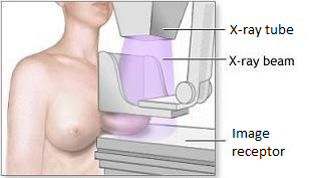
\includegraphics[width=0.5\textwidth,keepaspectratio]{figures/xraymammo.PNG} 
\caption[Mammographyc exam]{Mammographyc exam}
\label{fig:mammographyc ecam}
\end{figure} 

The mammography is used to detect parenchymal distortion, asymmetry, masses and clusters of microcalcifications within the breast.  These findings are not pathogenic
and require a tissue diagnosis to confirm the
presence of an invasive cancer, in situ cancer, or a nonmalignant finding. Microcalcifications are small calcium deposits embedded in a protein matrix .   They have x-ray attenuation coefficients substantially higher than breast tissue and therefore appear as bright spots in the x-ray images. The diameter of a microcalcification
is typically inferior to 1mm \citep{henrot_breast_2014}. In terms of form, breast microcalcifications can come in many shapes and sizes.  So, they can be round, linear, coarse or granular.  A mass is a radiological finding demonstrating an increased density versus the surrounding tissue. There is a large variation on mass size and shape, usually a suspicious mass is larger than 8mm and have irregular or speculated margins \citep{mckenna_abnormal_1994}.  Asymmetry and parenchymal distortion are visualised as tethering or indentation of breast tissue. They are the
third most common mammographic appearance of nonpalpable
breast cancer, representing nearly 6\% of abnormalities detected on screening mammography \citep{gaur_architectural_2013}. 

A standard mammographic protocol always includes breast compression prior to image acquisition. Women breast is compressed between two plates until a nearly uniform breast thickness is obtained. Nowadays, the European Commission recommends a force standardized breast compression, i.e. the compression stops at a level of force just below the subject’s pain threshold or to the maximum setting of the machine (not to exceed 200 N). Analog mammography used screen/film detector technology in order to display breast internal structures, thus a uniform breast compression was needed in order to ensure a uniform exposure over the breast volume. With digital mammography, the exposure variation could be corrected with post-processing, while the breast compression is still indispensable to hold the breast away from the chest wall, to reduce the blur due to physical motion, to reduce the absorbed dose of ionizing photons, to separate overlapping structures or to reduce image degrading scatter \citep{kopans2007breast}.


 
 %Breast cancer specialists estimate that breast cancer most frequently appears as microcalcifications and masses \citep{venkatesan_positive_2009}. 
Studies in different countries have assessed mammography sensitivity and specificity. The obtained sensitivities ranges between 81 and 88 \%, and the specificities between 83 and 98 \% \citep{kemp_comparing_2015,hofvind_sensitivity_2012}. The mammography sensitivity is mostly affected by dense breasts. A dense breast is a breast for which the  proportion of the fibroglandular tissues exceed greatly the proportion of fatty tissues. Fatty tissues are radiographically translucent, and lead to high intensity signal appearing on the mammographic images as dark areas. Meanwhile, the fibroglandular tissues and breast cancers tend to absorb more x-rays photons, therefore they will appear as white areas. The lack of contrast between the cancer and dense regions of the background make the detection more difficult.      
 
\subsection{Ultrasounds}\label{subsection:ultrasound}

Breast ultrasound uses high-frequency sound waves to image breast tissues. The ultrasound technician put gel on the skin above the area of interest and moves the sound-emitting probe over the skin. The emitted waves are bounced by the breast soft tissues. The probe picks up the reflected waves and transforms them into a 2D image. 

For asymptomatic women, a careful investigation of lateral and profound breast tissues is needed to identify the suspicious lesions. The limited field of view of the ultrasound image prevents from seeing abnormalities that lie deeper in the breast. Consequently, the ultrasounds are not sufficient for regular screening and are used to complement other screening tests. However, it is widely used to investigate suspicious lesions found within mammography, clinical or self-examinations. Breast ultrasound is particularly effective in differentiating  cysts from solid lesions. But has a low sensitivity for detection of microcalcifications which are the most common feature in addition to masses associated with breast cancer. Breast ultrasound can also be used for differential diagnosis, local staging and intervention guidance.

\textbf{Ultrasound elastography} is a sonographic imaging technique combining the ultrasound technology with the basic physical principles of elastography. Elastography assesses tissue deformability by providing information on the tissue elasticity. It consists of either an image of strain in response to force or an image of estimated elastic moduli. This approach is somehow equivalent to clinical or self-examination, but with a higher precision.

Shear-wave elastography uses focused pulses of ultrasound generated by the probe to induce soft tissues deformation. The tissues elasticity is assessed either by directly measuring soft tissues deformation or by measuring the speed of shear wave propagation. The combination of SWE with conventional ultrasound
increases the diagnostic performance for breast lesions, compared
with conventional ultrasound alone \citep{youk_shear_2017}.  Elastrography serves as a complementary tool to differentiate benign from malignant lesions by providing information about the lesion stiffness\citep{itoh_breast_2006,olgun_use_2014}
 
\subsection{Magnetic resonance imaging}\label{subsection:mri}

Magnetic resonance imaging (MRI) is a noninvasive procedure used in breast imaging for studying internal structure of the breast that cannot be properly visualized using standard mammography (dense breasts).  It employs radio-frequency waves and intense magnetic fields to excite hydrogen atoms. Body parts that contain hydrogen atoms (e.g. in water) are then imaged with contrasts depending on relaxation phenomenon characteristic of the tissues in the body. The quality of the image produced by MRI techniques depends, in part, on the strength of the received signal. For higher image quality, it is optimal to use an independent RF receiving coil placed in close proximity to the region of interest.  For breast imaging, dedicated breast MRI coils can be used. The patient is placed in prone position with the breast inside the coil and both arms by the sides of the body.

When the cancerous tumor develops, new vascularizations are created on the direct surrounding to provide oxygen.
Thus, for breast cancer imaging, a contrast agent may be used to enhance highly vascularized regions. These regions, corresponding to the lesions, are visualized due to their uptake of contrast agent. Contrast enhanced MRI is used as a screening modality for women with high risk of cancer.  

Low specificity and high cost of MRI restricts its use in a routine screening \citep{peters_meta_2008}. However, it is increasingly used for high-risk groups and for lesions that are difficult to detect with mammography or ultrasounds tests. 

\section{Conclusion}\label{section:conlusion}
Today, mammography is the primary imaging modality used in breast cancer screening and plays an important role in cancer diagnosis. Ultrasounds and Magnetic Resonance Imaging are complementary imaging techniques used mostly for dense breasts and high-risk women.
 
In order to obtain an accurate reading, the mammography machine needs to compress the breasts.  The discomfort and pain produced by breast compression might deter women from attending breast screening by mammography  \citep{aro_psychosocial_1999,fleming_intermittent_2013}. In a study by \citep{dullum_rates_2000} more than 50\% of attendants (N= 1800) mentioned from moderate to extreme physical discomfort.  It has been reported that the
fear for pain itself can already be a reason to avoid getting the first mammogram \citep{andrews_pain_2001}, and that 15\% of those who skipped the second appointment cited as the main cause an unpleasant or painful first mammogram \citep{fleming_intermittent_2013,whelehan_effect_2013}.  Postpone the mammographic exam can lead to delayed breast cancer diagnoses and worse prognoses (expected outcomes) for some women.

The main direct cause of pain in mammography is the flattening of the breast, which is directly linked to the applied compression force. Latest researches indicate that with a reduced level of compression (10N vs 30N), 24\% of women did not experience a difference in breast thickness. If breast thickness is not reduced when compression force is further applied, then discomfort increases with no benefit in image quality or average dose. Therefore, a detailed study on alternative breast compression techniques considering the patient comfort in addition to the image quality and ionizing radiation dose is needed.

The aim of this work is to provide a simulation framework capable to assess the patient physical comfort, as well as the corresponding image quality and average glandular dose for breast compression with different paddles designs. The developed numerical methods would serve to build an optimal compression paddle in terms of latter listed parameters, and therefore increase the adherence to breast cancer screening. 

In this scope, a subject-specific biomechanical Finite Element (FE\nomenclature{FE}{Finite Element}) model is developed and evaluated on real deformations measured on MR images. The proposed model is then used to compute the tissues deformation associated to breast compression during mammography.  The resulting internal stress/strain intensities are then used as a first estimate of the physical comfort. The deformed breast geometry is the subject of a Monte-Carlo image simulation allowing to assess the image quality (IQ\nomenclature{IQ}{Image Quality}) and average glandular dose (\nomenclature{AGD}{Average Glandular Dose}AGD), in order to validate the image quality for the different strategies of compression we are considering.




